\chapter{الگوریتم گرادیان کاهشی}
\section{شبه‌کد الگوریتم}
الگوریتم گرادیان کاهشی (Gradient Descent) یکی از پایه‌ای‌ترین روش‌های بهینه‌سازی مرتبه اول است. در \cref{alg:gd} شبه‌کد این الگوریتم آورده شده است:
\begin{algorithm}
	\caption{الگوریتم گرادیان کاهشی با گام ثابت}
	\label{alg:gd}
	\begin{algorithmic}[1]
		\Require تابع هدف \( f \)، نقطه شروع \( x_0 \)، نرخ یادگیری \( \alpha \)، معیار توقف \( \varepsilon \)
		\Ensure نقطه بهینه تقریبی \( x^* \)
		\State \( k \gets 0 \)
		\While{\(\|\nabla f(x_k)\| > \varepsilon\)}
		\State \( x_{k+1} \gets x_k - \alpha \nabla f(x_k) \)
		\State \( k \gets k+1 \)
		\EndWhile
		\State \Return \( x_k \)
	\end{algorithmic}
\end{algorithm}
در خطوط مختلف این الگوریتم به ترتیب مقداردهی اولیه، حلقه اصلی شرط توقف و به‌روزرسانی نقطه انجام می‌شود.

\section{فلوچارت الگوریتم}
فلوچارت زیر جزئیات الگوریتم \cref{alg:gd} را به صورت تصویری نمایش می‌دهد.
\begin{figure}[H]
	\centering
	\begin{tikzpicture}[node distance=1.3cm, auto, 
		block/.style={rectangle, draw, thick, text width=3cm, align=center, minimum height=0.8cm},
		decision/.style={diamond, draw, thick, text width=2.5cm, align=center, aspect=2}]
		\node[block] (start) {شروع};
		\node[block, below of=start] (init) {\( x_0, \alpha, \varepsilon \)};
		\node[decision, below of=init, yshift=-0.3cm] (cond) {\(\|\nabla f(x_k)\| > \varepsilon\)};
		\node[block, below of=cond, yshift=-0.7cm] (update) {\( x_{k+1} = x_k - \alpha \nabla f(x_k) \)};
		\node[block, below of=update] (inc) {\( k = k+1 \)};
		\node[block, below of=inc] (output) {خروجی \( x^* \)};
		\node[block, right of=cond, node distance=3.5cm] (stop) {پایان};
		\draw[->] (start) -- (init);
		\draw[->] (init) -- (cond);
		\draw[->] (cond) -- node[above] {بلی} (update);
		\draw[->] (cond) -- node[above] {خیر} (stop);
		\draw[->] (update) -- (inc);
		\draw[->] (inc) -- ++(0,-0.5) -| (cond);
	\end{tikzpicture}
	\caption{فلوچارت الگوریتم گرادیان کاهشی}
	\label{fig:gd-flowchart}
\end{figure}

\section{شکل با دو زیرشکل (رفتار الگوریتم)}
شکل \cref{fig:subfigures} دو وضعیت متفاوت همگرایی را نشان می‌دهد: (الف) نرخ یادگیری مناسب و (ب) نرخ یادگیری زیاد.
\begin{figure}[H]
	\centering
	\begin{subfigure}[b]{0.45\textwidth}
		\centering
		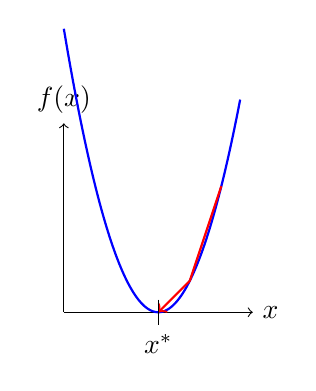
\begin{tikzpicture}[scale=0.8]
			\draw[->] (0,0) -- (3,0) node[right] {\(x\)};
			\draw[->] (0,0) -- (0,3) node[above] {\(f(x)\)};
			\draw[blue, thick, domain=0:2.8, samples=100] plot (\x, {2*(\x-1.5)^2});
			\draw[red, thick, ->] (2.5,{2*(2.5-1.5)^2}) -- (2,{2*(2-1.5)^2}) -- (1.5,{2*(1.5-1.5)^2});
			\draw (1.5,0.2) -- (1.5,-0.2) node[below] {\(x^*\)};
		\end{tikzpicture}
		\subcaption{نرخ یادگیری مناسب، همگرایی به نقطه بهینه}
		\label{fig:subfig-good}
	\end{subfigure}
	\hfill
	\begin{subfigure}[b]{0.45\textwidth}
		\centering
		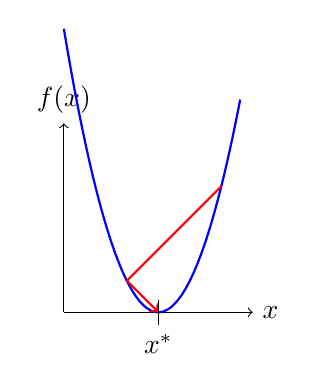
\begin{tikzpicture}[scale=0.8]
			\draw[->] (0,0) -- (3,0) node[right] {\(x\)};
			\draw[->] (0,0) -- (0,3) node[above] {\(f(x)\)};
			\draw[blue, thick, domain=0:2.8, samples=100] plot (\x, {2*(\x-1.5)^2});
			\draw[red, thick, ->] (2.5,{2*(2.5-1.5)^2}) -- (1,{2*(1-1.5)^2}) -- (1.5,{2*(1.5-1.5)^2});
			\draw (1.5,0.2) -- (1.5,-0.2) node[below] {\(x^*\)};
		\end{tikzpicture}
		\subcaption{نرخ یادگیری زیاد، نوسان قبل از همگرایی}
		\label{fig:subfig-bad}
	\end{subfigure}
	\caption{مقایسه رفتار الگوریتم گرادیان کاهشی با نرخ‌های یادگیری متفاوت}
	\label{fig:subfigures}
\end{figure}
در \cref{fig:subfigures} و زیرشکل‌های \subref{fig:subfig-good} و \subref{fig:subfig-bad} به ترتیب رفتار الگوریتم را مشاهده می‌کنید.

\section{جدول مقایسه روش‌ها}
جدول \cref{tab:optim-compare} ویژگی‌های سه روش بهینه‌سازی را مقایسه می‌کند. این جدول مطابق با خواسته‌های صورت‌مسئله طراحی شده است:
\begin{table}[H]
	\centering
	% تنظیم ارتفاع سلول به 10pt (فونت پایه 12pt)
	\setlength{\extrarowheight}{2pt}
	\renewcommand{\arraystretch}{0.833}
	\setlength{\tabcolsep}{4pt}
	% تعریف ستون با عرض 1.5cm و وسط‌چین
	\newcolunntype{M}[1]{>{\centering\arraybackslash}m{#1}}
	\begin{tabular}{|M{1.5cm}|M{1.5cm}|>{\columncolor{white}}M{1.5cm}|}  % موقتاً ستون سوم بدون رنگ
		\hline
		\rowcolor{gray!20}
		\textbf{روش} & \textbf{سرعت همگرایی} & \textbf{نیاز به مشتق} \\
		\noalign{\hrule height 1.2pt}  % خط ضخیم زیر هدر
		\rowcolor{blue!10} گرادیان کاهشی & خطی & بلی \\
		\hline
		\rowcolor{white} نیوتن & درجه د
		
		وم & بلی (هسین) \\
		\hline
		\rowcolor{blue!10} شبه‌نیوتن & ابرخطی & بلی (تقریب هسین) \\
		\hline
	\end{tabular}
	\caption{مقایسه روش‌های بهینه‌سازی مرتبه اول و دوم}
	\label{tab:optim-compare}
\end{table}
به ستون سوم در \cref{tab:optim-compare} دقت کنید که با یک خط ضخیم قرمز از بقیه جدا شده است.